\documentclass[11pt, a4paper, oneside]{article}

\usepackage[margin=3cm]{geometry}
\usepackage{graphicx} %Pretty documents
\usepackage{grffile} %Allow multi-dots in image names (otherwise first dot seen as file extension)
\graphicspath{{./images/}}
\usepackage{parskip} %No Indentation for Paragraphs
\usepackage[hidelinks]{hyperref} %Clickable PDF's
\usepackage{blindtext} %Use for text fillers and formatting
\usepackage{float} %Allow H in figures to fix position
\usepackage{siunitx} %Proper SI Units \SI{Value}{Units}
\usepackage{caption} %Allows caption*() to remove prefix for equations in figures
\usepackage{listings} %code

%Following Part makes each section on a new page
\let\stdsection\section
\renewcommand\section{\newpage\stdsection}

\title{\textsc{Session 1 Report - Group 03.1}
	\newline \textbf{EE3P11 - Electromagnetism Practical}\\
}
\author{
	\textsc{Rijk van Wijk | 4261569}\\
	and
	\textsc{Nicolaas du Plessis | 4203933}\\
	and
	\textsc{Paul Beckers | XXXXXXX}\\
	and
	\textsc{Jens Coppoolse | XXXXXXX}\\
	and
	\textsc{Michiel Desmedt | 4221095}\\
}
\date {\today}

\begin{document}
	\maketitle
	\thispagestyle{empty}
	\newpage
	
	\section*{Assignment 1: Frequency Domain Transmission Lines}
	\section*{Assignment 1: Frequency Domain Transmission Lines}

The first experiment was set-up as show below in figure \ref{fig:setup_1} and figure \ref{fig:setup_1_diagram}. From left to right, it consisted of a RF signal source, a signal generator, and an amplifier to modulate a \SI{1}{\kilo\hertz} square wave onto the RF signal source with a frequency of \SI{9.4756}{\giga\hertz}, which is then transmitted down the wave guide, past the slotted line detector, and to the load under investigation. The detector can then measure the amplitude variations over it's adjustable distance of the standing wave inside the wave guide, and display the signal on an oscilloscope (for qualitative representation) and a digital multimeter (for quantitative results). The oscilloscope show the \SI{1}{\kilo\hertz} modulated wave, with the amplitude representing that of the RF signal amplitude.

\begin{figure}[H]
	\centering
	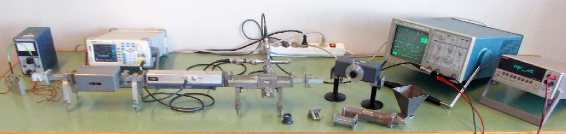
\includegraphics[width=\textwidth]{ass1_setup1.png}
	\caption{Experimental set-up for assignment 1 \cite[p.3]{lab_manual}}
	\label{fig:setup_1}
\end{figure}

\begin{figure}[H]
	\centering
	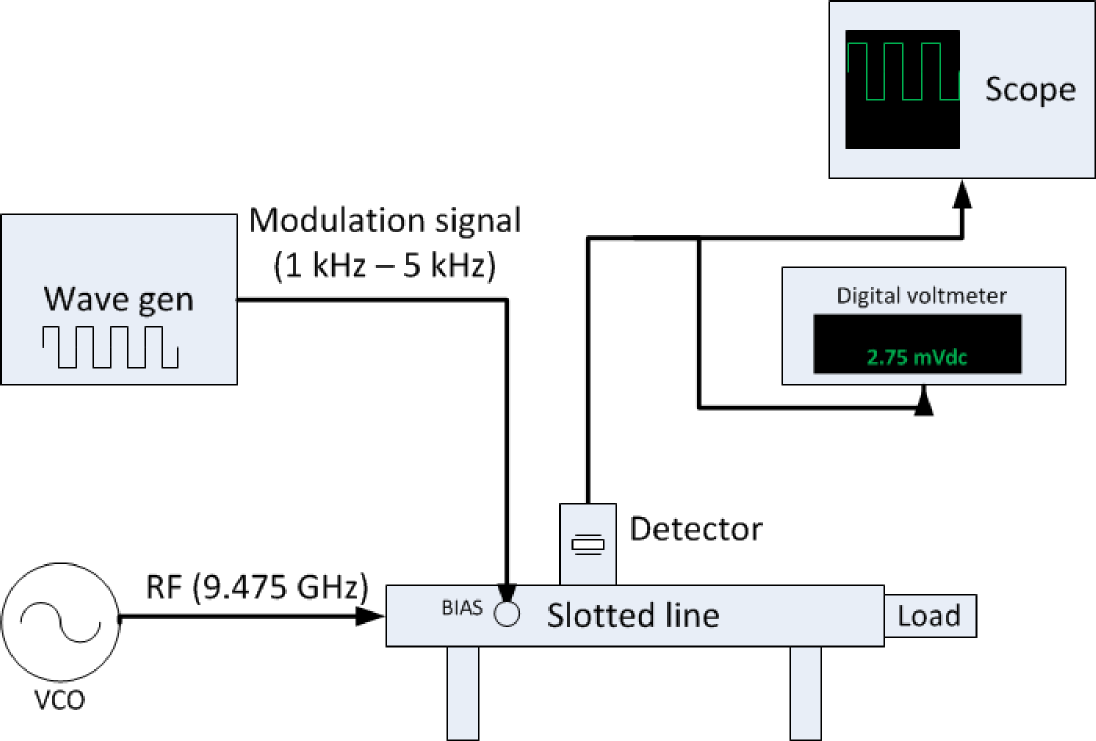
\includegraphics[width=\textwidth]{ass1_setup1_diagram.png}
	\caption{Diagram of experimental set-up for assignment 1}
	\label{fig:setup_1_diagram}
\end{figure}

The following questions were answered for the experimental set-up:

\subsection*{Wavelength}
The wavelength of the standing wave was determined by measuring the distance between the amplitude peaks on the slotted detector. By averaging three measurements, the final distance was \SI{2.2}{\centi\meter}, which is half the wavelength, giving a total wavelength of \SI{4.39}{\centi\meter}. The phase velocity is given by $v_{p} = \lambda \cdot f = 416 \cdot 10^6$ \SI {}{\meter\per\second} (1.39c).

The phase velocity represents the propagation speed of a single frequency component of the wave between to points. However, this information has little actual benefit, as it does not represent the propagation delay of the wave in the time domain. Instead, the value represents the distance and time between two consecutive phase occurrences in the standing wave. As two identical interference patterns can happen independent of each other, the interpreted speed of this occurrence (phase velocity) can be higher than the speed of light. As no information can be transmitted between these two points as this speed, this observation gives little usable information on the compound waveform.

\subsection*{Voltage-standing-wave ration (VSWR)}

Five different loads were compared, where the amplitudes of the maxima and minima of the standing wave were measured, and compared below in table \ref{table:results1}. For each load, the VSWR, the reflection coefficient $\Gamma$, and the delivered power to the load were calculated. Below are the formulas used for each value.

\begin{table}[h]
	\centering
	\begin{tabular}{|l|l|l|l|l|l|}
		\hline
		Load                   & $E_{min} (mV)$ & $E_{max} (mV)$ & VSWR     & $|\Gamma|$ & $P_{Load} (W)$  \\ \hline
		a) Open Waveguide      & 26.5    & 56.9    & 2.15     & 0.37       & $1.20 \cdot 10^{-3} / Z_0 $             \\ \hline
		b) Short Circuit 33 mm & 0       & 76.6    & $\infty$ & 1.00       & 0           \\ \hline
		b) Short Circuit 55 mm & 0       & 79.6    & $\infty$ & 1.00       & 0           \\ \hline
		c) Matched Load        & 41.7    & 46.5    & 1.12     & 0.057      & $1.27 \cdot 10^{-3} / Z_0 $            \\ \hline
		d) Horn Antenna        & 39.3    & 49.0    & 1.25     & 0.11       & $1.31 \cdot 10^{-3} / Z_0 $            \\ \hline
		
	\end{tabular}
	\caption{Results for different loads}
	\label{table:results1}
\end{table}

The VSWR is:
\begin{equation}
\label{eq:VSWR}
VSWR = \frac{|V_{max}|}{|V_{min}|}
\end{equation}

The reflection coefficient:
\begin{equation}
\label{eq:Gamma}
|\Gamma| = \frac{VSWR - 1}{VSWR + 1}
\end{equation}

The power delivered to the load is:
\begin{equation}
\label{eq:power}
P_{abs} = \frac{(V_0^+)^2}{2Z_0} (1 - |\Gamma|^2)
\end{equation}

\subsection*{Standing wave pattern comparison}
There is not measurable shift in the position of the nodes and anti-node between the 55mm and 33mm wave guide short circuits. The reason behind this is that the difference in the shorts is 22mm, which is have the calculated wavelength of the standing wave. Due to this, the observed standing wave in the detector has identical positions of the nodes and anti nodes.

\subsection*{X-band phase velocity}
For an electromagnetic wave in a wave guide, the wavelength is not the same as it would be in free space. The equation for the phase velocity is given below in equation \ref{eq:phase_vel}, where c is the speed of light, $\lambda$ is the wavelength, and a is the length of the wave guide

\begin{equation}
\label{eq:phase_vel}
v=\lambda f = \frac{c}{\sqrt{1-(\frac{\lambda}{2a})^2}}
\end{equation}

The wavelength of the EM wave must fit within the length of the wave guide, as it forms a standing wave between the two edges of the wave guide (as the body of the wave guide must be the same potential). Using the data from the experiment, we can plot the phase velocity for different frequencies in the X-band (\SI{8}{\giga\hertz} - \SI{12}{\giga\hertz}), as show below in figure \ref{fig:xband_phase_vel}

\begin{figure}[H]
	\begin{center}
		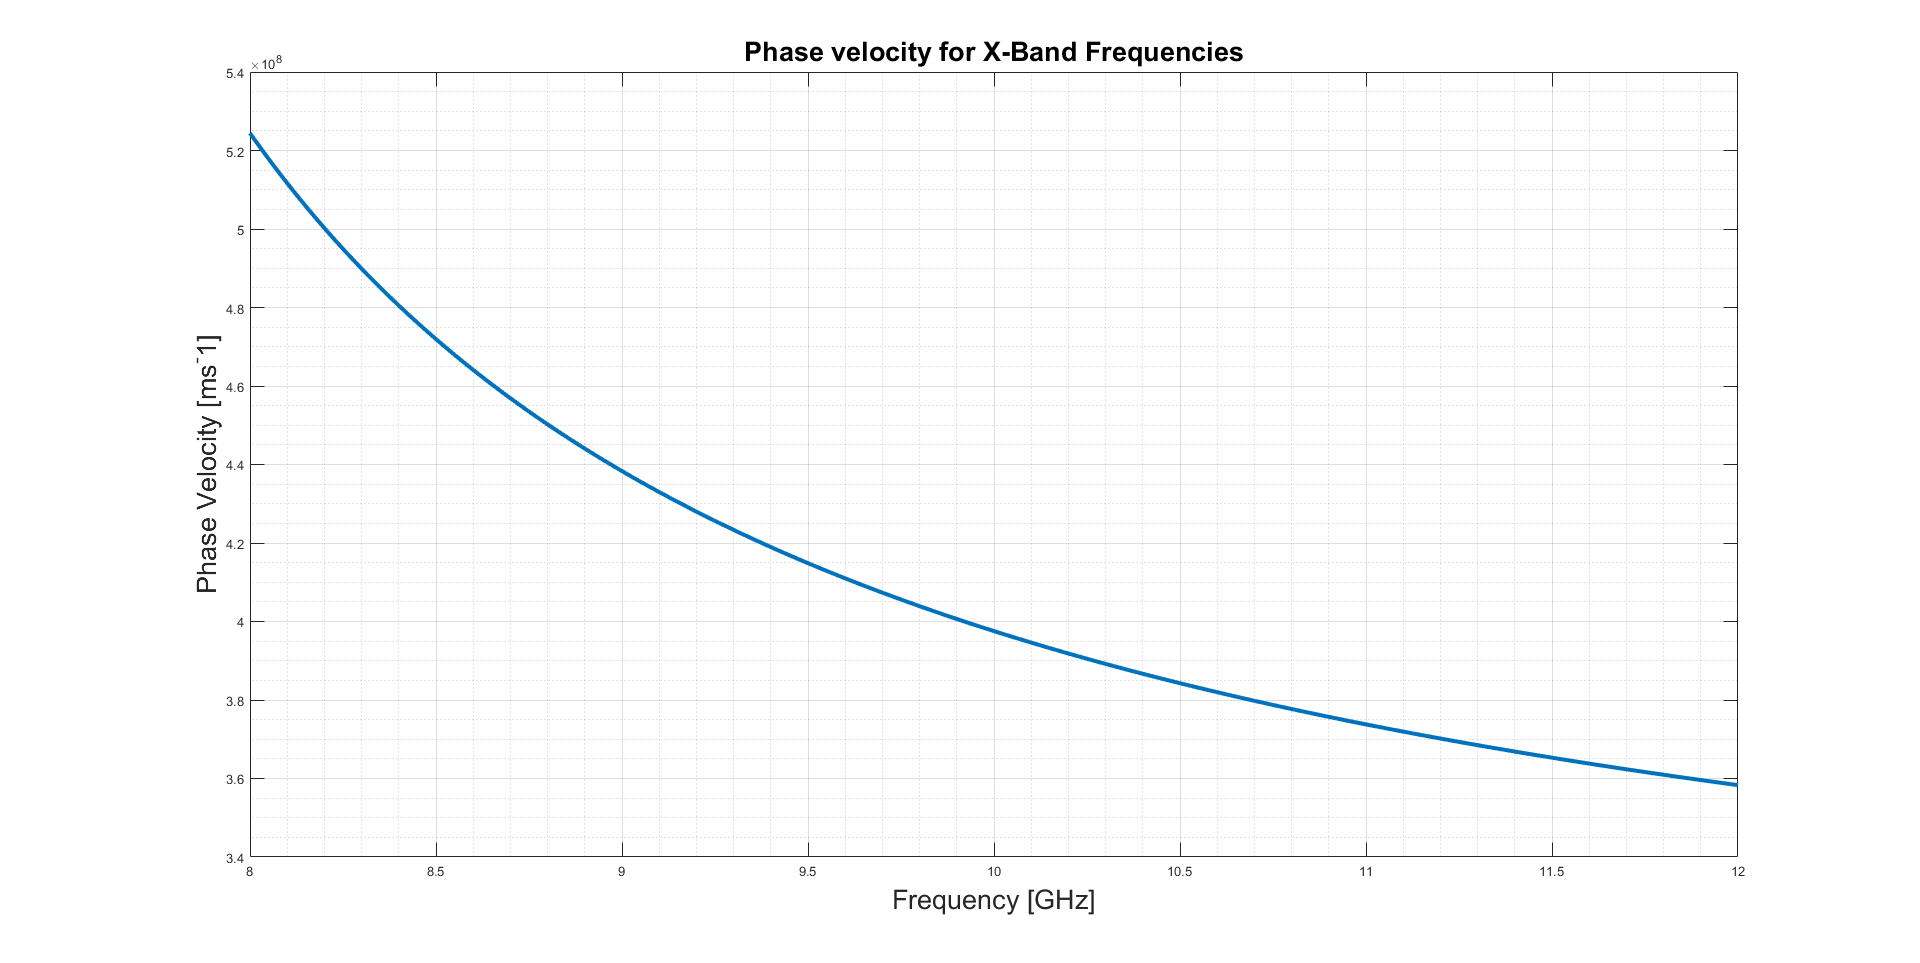
\includegraphics[width=\textwidth]{x_band_phase_velocity.png}
		\caption{X-Band phase velocities}
		\label{fig:xband_phase_vel}
	\end{center}
\end{figure}

\subsection*{Other parameters}
As the impedance of the loads can be calculated, using the measured values, the impedance of the wave guide can also be estimated. 

	\section*{Assignment 2: Time Domain Transmission Lines}
	\section*{Assignment 2: Time Domain Transmission Lines}

During this assignment, the setup in Figure \ref{fig:Ass2_setup} is used. It consists of a pulse generator which sends a square pulse to a DUT (device under test)via a coax cable (with $Z_0 = 50 \Omega$), a sampling unit, which samples the electric field in the coax cable, and an oscilloscope, which measures the sampled electric field strength.\\

\begin{figure}[h]
    \centering
    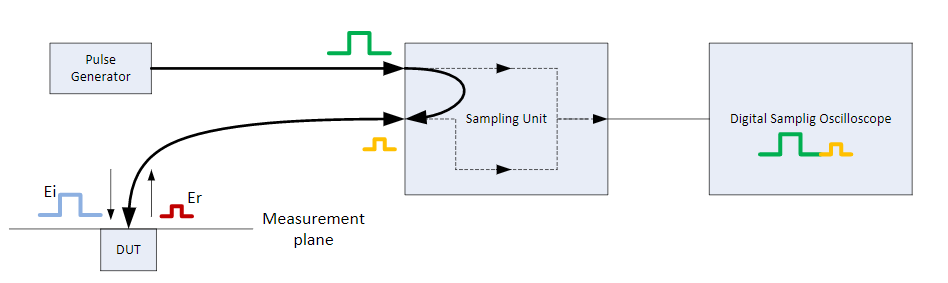
\includegraphics[width=1\textwidth]{Session1_files/Assignment2_setup.PNG}
    \caption{Experimental setup of Assignment 2}
    \label{fig:Ass2_setup}
\end{figure}

\subsection*{Part 1. Time Domain Reflectometry}

In this part, the reflection of an incident square pulse is investigated. As the oscilloscope will measure the total electric field in the coax cable, it will also register the reflection of the pulse, from which the reflection coefficient can be derived.


	

	\section*{Appendix}
	\begin{thebibliography}{99}

\bibitem{lab_manual} Blackboard Lab Manual. (2017). EE3P11 - EM Practicum, 2016-2017 Q3.


\end{thebibliography}

\section*{Appendix} 


\end{document}